\documentclass[10pt,twocolumn]{article}
\usepackage[a4paper,margin=1.45cm,columnsep=0.55cm]{geometry}
\usepackage[T1]{fontenc}
\usepackage{lmodern}
\usepackage{amsmath,amssymb}
\usepackage{graphicx}
\usepackage{booktabs}
\usepackage{microtype}
\usepackage[hidelinks]{hyperref}
\usepackage{titlesec}
\usepackage{enumitem}
\titlespacing*{\section}{0pt}{5pt}{2pt}
\titleformat*{\section}{\normalsize\bfseries}
\setlength{\parskip}{0pt}
\setlist{nosep,leftmargin=1.1em}
\newcommand{\NQAOAruns}{2\,016}
\newcommand{\NEvals}{187\,303}
\newcommand{\NLargeRuns}{2\,928}
\newcommand{\NLargeInstances}{216}
\newcommand{\VQZYequal}{78}
\newcommand{\COBYLAequal}{0.36}
\newcommand{\LRgainEqual}{3.9}
\newcommand{\LRgainShare}{1.9}
\newcommand{\LRgainUniformCPU}{22}
\newcommand{\COBYLAshare}{2.6}
\newcommand{\NoiseLR}{0.42}
\newcommand{\IdealLR}{0.78}
\newcommand{\ScLocalTwelveEq}{86}
\newcommand{\ScCobylaTwelveEq}{92}
\newcommand{\ScCobylaTwentyEq}{2}
\newcommand{\ScSpectralTwentyEq}{50}
\newcommand{\ScLocalTwentyEq}{18}
\newcommand{\ScCobylaTwentyCpu}{21}
\newcommand{\ScSpectralTwentyCpu}{100}
\newcommand{\ScLocalTwentyCpu}{77}
\newcommand{\AblFields}{0.30}
\newcommand{\AblCouplings}{0.01}
\newcommand{\VQZYcircuits}{6\,473}
\newcommand{\RuntimeSpread}{2.9}
\newcommand{\VQLApEq}{0.965}
\newcommand{\VQLApCpu}{0.981}
\newcommand{\VQLnearMax}{$<$0.01}
\newcommand{\COBYLAtotal}{196\,556}
\newcommand{\VQZYtotal}{8\,675\,556}
\newcommand{\NIonQ}{12}
\newcommand{\TriMin}{1\,670}
\newcommand{\TriMax}{2\,166}
\newcommand{\MeshDiffer}{4}
\newcommand{\MeshTotal}{9}
\newcommand{\PoolDevices}{8}
\newcommand{\PoolFastTime}{9.4}
\newcommand{\PoolFastEnergy}{27.3}
\newcommand{\PoolNightTime}{11.8}
\newcommand{\PoolNightEnergy}{23.7}
\newcommand{\PoolEcoTime}{13.4}
\newcommand{\PoolEcoEnergy}{22.0}
\newcommand{\PoolNaiveTime}{37.5}
\newcommand{\PoolNaiveEnergy}{56.1}
\newcommand{\PoolNightLimit}{12}

\newcommand{\TableNtwelve}{%
Uniform random sampling & 0 & 0 & 0.07 & 48 & 0.04 & 29 \\
Random with target share & 0 & 0 & 0.07 & 48 & 0.41 & 74 \\
Simulated annealing & 0 & 0 & -- & 64 & -- & 87 \\
Local search (restarts) & 0 & 0 & -- & 84 & -- & 100 \\
Spectral bisection & 0 & 0 & -- & 67 & -- & 100 \\
\midrule
LR-QAOA, $p=2$ & 132 & 0 & 0.27 & 85 & 0.78 & 99 \\
QAOA + COBYLA, $p=2$ & 132 & 200 & 0.36 & 94 & 1.1 & 100 \\
CVaR-QAOA + COBYLA, $p=2$ & 132 & 31 & 0.31 & 90 & 0.87 & 99 \\
Warm start (spectral)$^\dagger$, $p=2$ & 132 & 200 & 7.8 & 94 & 21 & 100 \\
\midrule
varQITE ZY (paper, all pairs) & 66 & 8\,675 & 78 & 100 & $<$0.01 & $<$0.01 \\
varQITE A (all pairs) & 66 & 7\,566 & 24 & 33 & $<$0.01 & 0.01 \\
varQITE A$^{+}$ (edges, our ext.) & 22 & 5\,003 & $<$0.01 & $<$0.01 & $<$0.01 & $<$0.01 \\
varQITE B (IonQ-native, edges) & 22 & 4\,686 & 0.01 & 13 & 0.01 & 7.8 \\
}


\title{\vspace{-1.1cm}\large\bfseries Quantum optimisation for heterogeneous mesh partitioning:\\an open, exactly graded benchmark of QAOA and varQITE\vspace{-0.25cm}}
\author{\normalsize Team ZollerQu --- Qollab $\times$ IonQ Hackathon, October 2026}
\date{\vspace{-0.75cm}}

\begin{document}
\maketitle

\noindent\textbf{Abstract.} Parallel PDE solvers split a mesh between compute devices; on heterogeneous clusters each device should receive work in proportion to its speed while the cut between parts stays short. We cast this two-device split with a target work share $\alpha$ as an Ising problem and benchmark quantum samplers against classical heuristics on nine reproducible finite-element meshes (12--24 coarse regions, one qubit each), grading every method against the exact optimum. In noiseless simulation, QAOA beats random sampling ($\LRgainEqual\times$ per shot at $\alpha{=}0.5$; $\LRgainShare\times$ the fair target-share sampler at $\alpha{=}0.8$) and matches local search at 12 qubits, but falls far behind classical methods at 16--20 qubits. IonQ's varQITE reaches a near-optimal split on $\VQZYequal\%$ of shots at $\alpha{=}0.5$, yet fails at $\alpha{=}0.8$ because of a structural limit of its ansatz that we identify. We claim no quantum advantage.

\section{Introduction}
Graph partitioning of finite-element meshes decides load balance and communication in parallel solvers. IonQ with Ansys/Synopsys recently inserted quantum graph partitioning into LS-DYNA to reduce fill-in of sparse direct solvers, using varQITE \cite{aboumrad2025} and Iterative-QAOA \cite{zhu2026}, always with \emph{balanced} halves and closed code; quantum annealing has been tried for HPC load balancing \cite{qaLB2024}. We study the \emph{heterogeneous} case (unequal device speeds, hence unequal target shares), release all code, and grade every quantum and classical method against exact enumeration on the same objective.

\section{Problem, benchmark and model}
\textbf{Benchmark.} Nine plates meshed with Delaunay triangulation (1\,670--2\,166 triangles): a rectangle with a known answer, an L-plate with a heat source, two sources, a plate with a hole (stress-style mesh), and a five-step complexity ladder on one L-plate (uniform $\to$ three sources $\to$ heavy-material zone with $3\times$ work $\to$ strong-coupling zone with $3\times$ border cost $\to$ priority zone). Each mesh is grouped into $n$ connected regions by $k$-means with a connectivity repair; region work and border cost are summed exactly.

\textbf{Ising model.} With $z_i{=}{+}1$ (device A) or ${-}1$ (device B), normalised work $\tilde a_i$ and border costs $\tilde c_{ij}$,
\begin{equation*}
E(z)=\sum_{\langle ij\rangle}\tilde c_{ij}\tfrac{1-z_iz_j}{2}+\lambda\Big(\sum_i\tilde a_iz_i-(1-2\alpha)\Big)^{2}\;[+\mu P(z)],
\end{equation*}
following the Ising form of graph partitioning \cite{lucas2014}. The balance term couples \emph{every} pair of regions ($n(n{-}1)/2$ two-qubit terms), which suits IonQ's all-to-all connectivity. Scenarios: two equal devices ($\alpha{=}0.5$, $\lambda{=}10$) and CPU+GPU with an assumed $4\times$ faster GPU ($\alpha{=}0.8$, $\lambda{=}3.98$); $\lambda$ is shared per scenario and selected by exact enumeration. A synthetic 8-device pool (CPUs/GPUs with speed, memory and power) shows the device-choice layer: fastest plan 9.4\,h/27.3\,kWh, overnight 11.8\,h/23.7\,kWh, lowest energy 13.4\,h/22.0\,kWh, versus 37.5\,h/56.1\,kWh for equal shares (modelled, not measured).

\section{Methods}
\textbf{Quantum (noiseless statevector, cross-checked with Qiskit to $10^{-15}$).} QAOA with cost layer $e^{-i\gamma E}$ and mixer $e^{+i\beta\sum X}$: linear-ramp LR-QAOA \cite{lrqaoa2025}; optimised angles with COBYLA, Nelder--Mead, Powell, L-BFGS-B (budget 200 evaluations) and shot-based SPSA \cite{spall1998}; CVaR-QAOA \cite{cvar2020}; warm starts \cite{egger2021}; a symmetry-reduced variant. varQITE \cite{morris2024}: each step solves $G\,\dot\theta=d$ with $d_k={-}(\langle P_kH\rangle-\langle P_k\rangle\langle H\rangle)$ and $G_{kj}{=}\partial\langle P_k\rangle/\partial\theta_j$ by parameter shift, for the paper's $e^{i\theta Z_rY_q}$ ansatz on all pairs (ZY), a $R_Y$+CX ansatz on all pairs or graph edges (A), our extension with one $R_Y$ per qubit (A$^+$) and an IonQ-native RZZ+RX ansatz (B), all trained on exact expectations.
\textbf{Classical.} Uniform and target-share random sampling, simulated annealing, local search with restarts, spectral bisection; same objective, same budget of 1\,000 candidates as QAOA's 1\,000 shots.
\textbf{Honesty measures.} All schedules, step sizes and annealing temperatures are tuned on separate calibration meshes, never on scored instances; the p=0 control and the target-share sampler are always reported; the main metric is the probability of a split with cost $\le1.05\times$ optimum; 30 injected bugs (signs, bit order, schedules, metric formulas) are all caught by the cell's checks; a crude depolarising estimate $F{=}(1{-}0.005)^{N_{2q}}$ indicates noise sensitivity.

\begin{figure*}[t]
\centering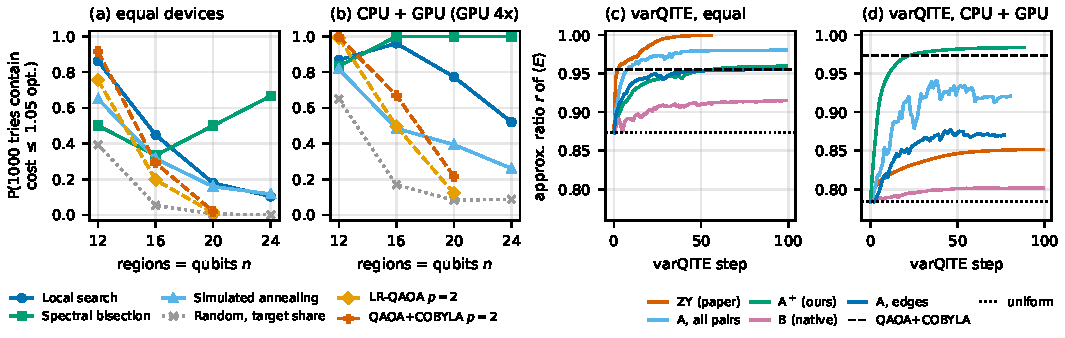
\includegraphics[width=\textwidth]{fig_results.pdf}\vspace{-0.25cm}
\caption{(a,b) Probability that 1\,000 candidates (classical) or shots (QAOA, noiseless) contain a split within 5\% of the optimum, versus problem size (cases 2 and 9, seeds 7--9; the 24-qubit reference is the best classical result; QAOA is not simulated at 24 qubits). (c,d) varQITE training curves at $n{=}12$ (mean over nine cases), with QAOA+COBYLA and uniform sampling for reference.}
\label{fig:results}\vspace{-0.15cm}
\end{figure*}

\begin{table*}[t]
\centering\footnotesize
\caption{Results at $n{=}12$ qubits (nine cases, noiseless): two-qubit gates, training circuits, per-shot probability of cost $\le1.05\times$ optimum (\%), and probability that 1\,000 shots/candidates contain such a split (\%). $^\dagger$Starts from the classical spectral split.}
\label{tab:n12}\vspace{0.05cm}
\begin{tabular}{@{}lrrrrrr@{}}
\toprule
& & & \multicolumn{2}{c}{equal devices ($\alpha{=}0.5$)} & \multicolumn{2}{c}{CPU+GPU ($\alpha{=}0.8$)}\\
\cmidrule(lr){4-5}\cmidrule(l){6-7}
Method & 2q gates & training circuits & per shot & hit@1000 & per shot & hit@1000\\
\midrule
\TableNtwelve
\bottomrule
\end{tabular}\vspace{-0.3cm}
\end{table*}

\section{Results}
\textbf{12 qubits (Table~\ref{tab:n12}).} All QAOA variants beat random sampling on every case: LR-QAOA raises the per-shot success $\LRgainEqual\times$ at $\alpha{=}0.5$; at $\alpha{=}0.8$ it is $\LRgainUniformCPU\times$ uniform guessing but only $\LRgainShare\times$ the classical target-share sampler (QAOA+COBYLA $\COBYLAshare\times$). An ablation explains the gap: the single-region terms alone give $\AblFields\%$ per shot, the pair terms alone $\AblCouplings\%$, both $\IdealLR\%$. With 1\,000 shots QAOA matches the best classical heuristic (local search $\ScLocalTwelveEq\%$, QAOA+COBYLA $\ScCobylaTwelveEq\%$ at $\alpha{=}0.5$), but at 4\,096 states exhaustive search is exact and cheap. Warm starts inherit most of their success from the spectral split; the convex-relaxation warm start is degenerate here ($c_i{=}\alpha$ for every region).

\textbf{Scaling (Fig.~\ref{fig:results}a,b; 216 instances, \NLargeRuns\ QAOA runs on a Hetzner node).} At fixed depth $p{=}2$ QAOA loses about an order of magnitude per shot for every four extra qubits. At 20 qubits QAOA+COBYLA finds a split within 5\% in $\ScCobylaTwentyEq\%$ / $\ScCobylaTwentyCpu\%$ of runs ($\alpha{=}0.5$ / $0.8$), versus $\ScSpectralTwentyEq\%$ / $\ScSpectralTwentyCpu\%$ for spectral bisection and $\ScLocalTwentyEq\%$ / $\ScLocalTwentyCpu\%$ for local search.

\textbf{varQITE (Fig.~\ref{fig:results}c,d).} At $\alpha{=}0.5$ the paper's ZY ansatz converges to near-optimal splits ($\VQZYequal\%$ per shot, 30--100\% on every case) with 66 two-qubit gates, but only after $\approx\VQZYcircuits$ exact-expectation training circuits. At $\alpha{=}0.8$ every varQITE variant fails: in ansatz A and ZY a qubit that is only ever a control keeps a 50/50 marginal for all angles, which caps a unique optimum at probability $1/2$; A$^+$ removes the cap and reaches $r{\approx}0.98$ but still misses the 5\% window. Graph-edge versions (22 gates) are too weak.

\textbf{Noise and outcome.} The depolarising estimate lowers LR-QAOA ($p{=}2$, $\alpha{=}0.8$) from $\IdealLR\%$ to $\NoiseLR\%$ per shot and makes deeper circuits worse. The modelled runtime of every method's best split lies within $\RuntimeSpread\%$ of the runtime-optimal split.

\section{Discussion and limitations}
The pipeline works end to end and quantifies where today's quantum samplers stand on a real engineering objective: competitive at 12 qubits, outpaced by classical heuristics beyond, and---for varQITE---strongly dependent on ansatz structure under unequal shares. All results are noiseless simulations or models; varQITE training used exact expectations; runtimes, energies and device speeds are modelled assumptions. At 16 qubits the graph-edge varQITE variants still never reach the 5\% window. Four of the nine meshes (cases 1, 2, 4, 5) differ at bit level between the macOS/arm64 and Linux/x86-64 builds, so the server's large-mode case-2 instances are equivalent but not identical to the notebook's; shipping meshes as data files will fix this. Next: the single batched IonQ Forte~1 noise-model run (p=0 control, QAOA and the final trained varQITE circuits), and measured CPU/GPU runs of refined meshes on HPC.

\noindent\textbf{This effort is supported by Qollab \& IonQ.} Code and all result files: \url{https://github.com/Oussema-t/zollerqu-qollab} (branch \texttt{mesh}). AI assistants (Claude Code, ChatGPT) were used for code and text; every number is produced by the published code.

{\footnotesize
\begin{thebibliography}{9}\setlength{\itemsep}{0pt}
\bibitem{aboumrad2025} W.~Aboumrad \emph{et al.}, Accelerating large-scale linear algebra using variational quantum imaginary time evolution, arXiv:2503.13128 (2025).
\bibitem{zhu2026} D.~Zhu \emph{et al.}, End-to-end performance of quantum-accelerated large-scale linear algebra workflows, arXiv:2603.15515 (2026).
\bibitem{qaLB2024} Load balancing for high performance computing using quantum annealing, arXiv:2408.04097 (2024).
\bibitem{lucas2014} A.~Lucas, Ising formulations of many NP problems, Front.\ Phys.\ \textbf{2}, 5 (2014).
\bibitem{lrqaoa2025} J.~A.~Monta\~nez-Barrera, K.~Michielsen, Toward a linear-ramp QAOA protocol, npj Quantum Inf.\ \textbf{11}, 131 (2025).
\bibitem{spall1998} J.~C.~Spall, Implementation of the simultaneous perturbation algorithm, IEEE Trans.\ Aerosp.\ Electron.\ Syst.\ \textbf{34}, 817 (1998).
\bibitem{cvar2020} P.~Kl.~Barkoutsos \emph{et al.}, Improving variational quantum optimization using CVaR, Quantum \textbf{4}, 256 (2020).
\bibitem{egger2021} D.~J.~Egger, J.~Mare\v{c}ek, S.~Woerner, Warm-starting quantum optimization, Quantum \textbf{5}, 479 (2021).
\bibitem{morris2024} T.~D.~Morris, A.~Kaushik, M.~Roetteler, P.~C.~Lotshaw, Performant near-term quantum combinatorial optimization, arXiv:2404.16135 (2024).
\end{thebibliography}}
\end{document}
